\section{Background}
In this section we will discuss the background of the two JIT compiler frameworks we are interested in: LLVM MCJIT and OMR JitBuilder.
In particular, we will focus on the motivation for each framework, as well as discuss the techniques and features they provide.
\section{LLVM}
\label{sec:llvm}
LLVM, which at one time stood for Low Level Virtual Machine, is a popular set of open-source, modular compiler and toolchain components \cite{lattner2004llvm}.
The compiler framework was originally designed to provide analysis and transformation for an application throughout it's entire lifetime: from initial compilation and linking, through to runtime and even while the application was offline (see Figure \ref{fig:llvmarch}).
\begin{figure*}
    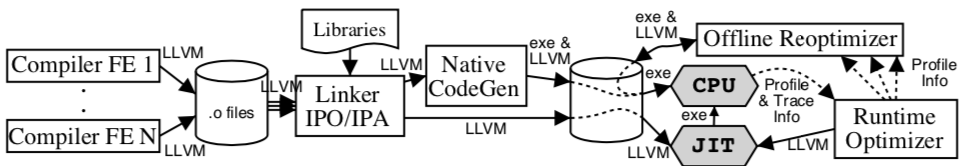
\includegraphics[width=\textwidth]{images/llvm-architecture.png}
    \caption{ The LLVM Compiler Framework Architecture \cite{lattner2004llvm}.}
    \label{fig:llvmarch}
    \Description[]{}
\end{figure*}
To achieve this ambitious goal, the framework utilizes a well defined, human-readable, intermediate representation called LLVM IR.
The IR, which is initially generated by the front end can be packaged with the target architecture binary along with profiling instructions for later runtime compilation (JIT) as well as more aggressive offline optimizations, provides a number of characteristics:
\begin{itemize}
    \item The IR maintains Static Single Assignment (SSA) form with unlimited virtual registers.
    \item Each register is of one of four primitive types: boolean, integer, floating-point or pointer.
    \item Similar to RISC, memory operations are carried out in registers, and between registers and memory using Load and Store instructions.
    \item The IR is limited to 31 opcodes.
    \item The IR is organized into basic blocks which must be composed of valid control flow graphs, simplifying the work required for various optimizations. 
\end{itemize}

\begin{lstlisting}[float,floatplacement=H,
caption={LLVM IR for a function multiplying x * y and adding z \cite{LLVM_Jit_Tutorial}},
label=lst:llvm_ir]
define i32 @mul_add(i32 %x, i32 %y, i32 %z) {
    entry:
    %tmp = mul i32 %x, %y
    %tmp2 = add i32 %tmp, %z
    ret i32 %tmp2
}\end{lstlisting}

This report will focus on LLVM's JIT framework - MCJIT.


\section{JitBuilder}
\label{sec:jitbuilder}
JITBuilder.